\chapter{Materiais e Métodos}
\label{chap:mat}
asdfasdfsdf

%--------- NEW SECTION ----------------------
\section{Lista de componentes}
\label{sec:espc}
%\subsection{Estrutura analítica do protótipo}
%\label{ssec:pbs}
%asdkjfsdalkjf
Para a confeção do sistema de percepção foi necessário a aquisição dos seguintes itens:
\begin{table}[]
\centering
\begin{tabular}{|l|l|l|l|}
\hline
{Item}                           & {Qtd.} & {Preço Unit.} & {Preço Total}  \\ \hline
Phidgets Interface Kit 8/8/8     & 1  & R\$ 271,82  & R\$ 271,82  \\ \hline
Nucleo STM32F401RE               & 1  & R\$ 43,287  & R\$ 43,287  \\ \hline
Sensor de Proximidade BCBI5770   & 5  & R\$ 36,90   & R\$ 184,50  \\ \hline
Maz-Sonar EZ1                    & 1  & R\$ 101,76  & R\$ 101,76  \\ \hline
IMU XSENS MTi 1                  & 1  & R\$ 1597,5  & R\$ 1597,5  \\ \hline
GPS Swiftnav Piksi 1.3.2         & 1  & R\$ 3398,0  & R\$ 3398,0  \\ \hline
Sensor de Temperatura LM35       & 1  & R\$ 5,75    & R\$ 5,75    \\ \hline
Câmera LWIR Lepton FLIR          & 1  & R\$ 812,05  & R\$ 812,05  \\ \hline
Phidgets Current Sensor          & 3  & R\$ 105,329 & R\$ 315,98  \\ \hline
NUC5i5RYK                        & 1  & R\$ 1380,83 & R\$ 1380,83 \\ \hline
Smart Charger EB325A             & 1  & R\$ 2200,00 & R\$ 2200,00 \\ \hline
Placa de Gerenciamento de Energia & 1 & R\$ 1004,16 & R\$ 1004,16 \\ \hline
Baterias DSNH2054HD34            & 2  & R\$ 1004,16 & R\$ 2008,32 \\ \hline
Nucleo STM32L432KC                      & 1  & R\$ 20,20   & R\$ 20,20   \\ \hline
\end{tabular}

\caption{Lista de Componentes}
\end{table}
\pagebreak
Todos os itens já estavam disponíveis para uso na área de robótica. A única excessão foram os sensores de proximidade, os quais tiveram que ser comprados.



%--------- NEW SECTION ----------------------
\section{Diagramas mecânicos}
\label{sec:diagm}

\subsection{Suportes para os componentes internos do robô}

Para fixar todos os sensores e componentes eletrônicos de maneira organizada, foi desenhado uma estrutura em forma de prateleira, na qual é possível anexa-los. As peças foram impressas em uma impressora 3D de forma que seja possível encaixa-las uma nas outras para facilitar o desenvolvimento. Essa peça irá ficar no compartimento superior da housing do robô.

Na Fig. \ref{Prateleira} é possível observar três peças empilhadas e na Fig. \ref{Prateleiracsensor} se vê a mesma com os sensores presos.

    \begin{figure}[H]
	\centering
	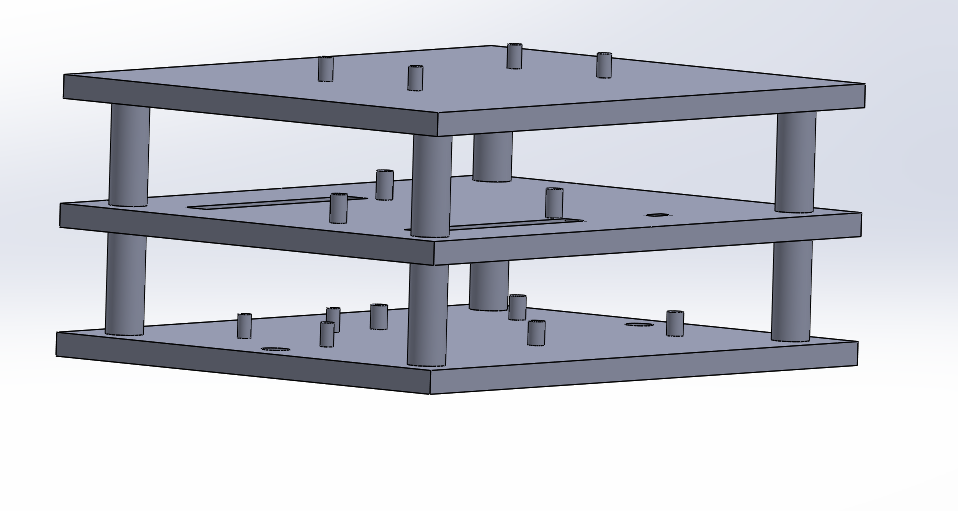
\includegraphics[width=14cm]{Figures/prateleira.png}
	\caption{Prateleira para suporte dos componentes eletrônicos} \label{Prateleira}
	\end{figure}
	
	\begin{figure}[H]
	\centering
	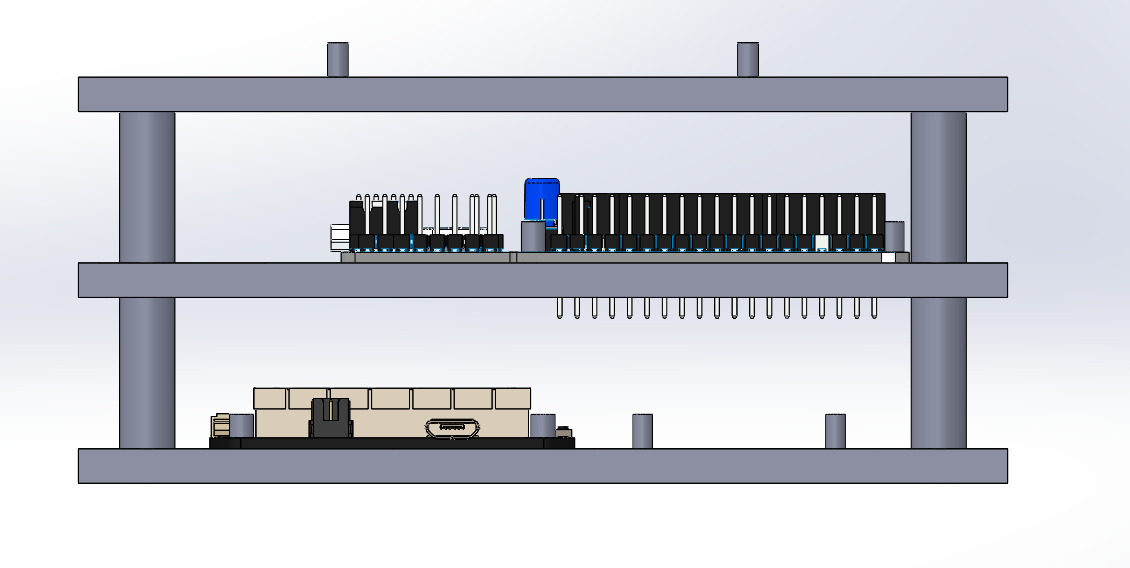
\includegraphics[width=16cm]{Figures/prateleiracsensores.png}
	\caption{Prateleira para suporte com sensores} \label{Prateleiracsensor}
	\end{figure}

O compartimento inferior da housing será utilizada para os componentes relacionados a energização do robô. Isso inclui as baterias, carregador inteligente e a placa de gerenciamento de energia. Para a fixação desses componentes foi desenvolvida a seguinta peça.

	\begin{figure}[H]
	\centering
	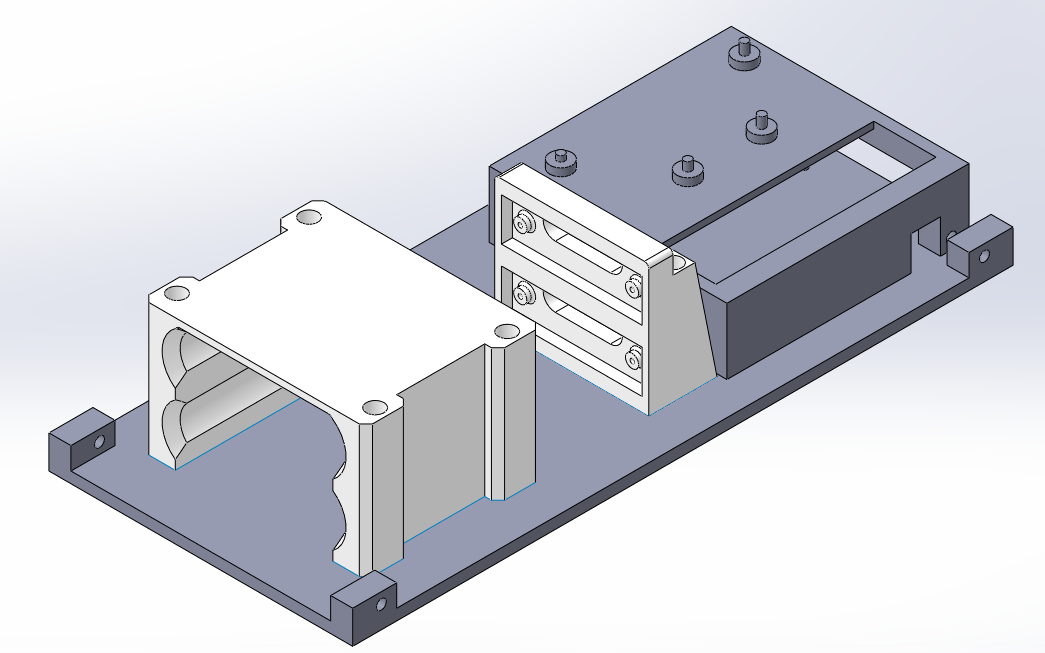
\includegraphics[width=14cm]{Figures/pecadebaixo.png}
	\caption{Prateleira para suporte dos componentes de alimentação} \label{pecaaliment}
	\end{figure}
	
	Todos os componentes serão fixados na estrutura do robô sem realizar nenhum furo ou alteração na mesma.
%--------- NEW SECTION ----------------------
\section{Modelo esquemático de alimentação e comunicação}
\label{sec:modesq}

A alimentação do sistema é proveniente de duas baterias LiPo que fornecem tensão de 14V. Todo o gerenciamento de energia do sistema é feita pela Power Management Board, esta placa é responsável por distribuir a alimentação de entrada para os demais subsistemas da Perception. 

A placa de interface Phidgets além de funcionar como hub para uma grande parte dos sensores também é responsável por compatibilizar o nível de tensão para os equipamentos eletrônicos, fornecendo 5V para as placas microprocessadas, sensores e a alimentação de todas as USBs. 

A comunicação entre os sistemas da Perception na maior parte acontecem através da Phidgets, já que ela concentra as informações uriundas de suas portas USB, entrada digitais e entradas analógicas em uma única porta USB para a NUC. Porém, a câmera térmica e a comunicação com os dynamixels acontecem de forma independente. Estes possuem portas USBs dedicadas na NUC.

O esquemático de alimentação e comunicação entre todos os elementos do sistema de Percepção está disponibilizado no apêndice XX.

\subsection{Diagramas elétricos}
\label{sec:diage}
O diagrama elétrico do sistema está disponível no apêndice XX. Neste diagrama encontram-se todas as conexões elétricas e de comunicação bem como as especificações de conectores e cabos utilizados no projeto. 

\subsection{Esquemas eletrônicos}
\label{ssec:esqe}

O único esquemático eletrônico realizado pela equipe da Perception foi uma placa hub de 5V para poder alimentar os sensores de proximidade visto que a Phidgets possui apenas umas saída de 5V disponibilizada. Nesta placa foram colocados os pin header para cada sensor de proximidade, fornecendo 5V, GND e os pinos digitais dos sensores foram disponibilizados em um conector Molex para facilitar o cabeamento entre o hub e a Phidgets.

O esquemático eletrônico e board estão mostrados no anexo XX.

%--------- NEW SECTION ----------------------
\section{Especificação das funcionalidades}
\label{sec:espf}
asdfadsfsdfs

%\subsection{Fluxo das informações}
%\label{ssec:fluxo}
%asdfsaf

\subsection{Aquisição}
\label{ssec:func1}
    \subsubsection{Objetivo}
    Realizar a comunicação e a aquisição dos dados provinientes da câmera térmica, sensores de proximidade, sonar, GPS, IMU, sensor de temperatura, placa multiplexadora de bateria e sensores de corrente.
        
     \subsubsection{Dependências}
     Esta funcionalidade não é dependente de nenhum outro processo.
    
     \subsubsection{Premissas}
     	\begin{itemize}
        	\item A interface microcontrolada Nucleo STM32F401RE deve estar com firmware embarcado para conversão de dados SPI para UART.
            \item A câmera térmica deverá estar conectada à interface Nucleo STM32F401RE
            \item A câmera stereo deve está conectada à NUC através da porta USB
            \item O sensores de temperatura, corrente e sonar devem estar conectados as entradas analógicas da interface Phidgets
            \item O sensor de proximidade deve está conectado a entrada digital da interface Phidgets
            \item O GPS e a IMU devem estar conectados a portas USB da Phidgets
            \item As placas de interface devem estar energizadas.
        \end{itemize}
     
     \subsubsection{Descrição da Funcionalidade}
        	 \indent O processo de aquisição de dados envolve a comunicação dos sensores com seus respectivos drivers no ambiente ROS e a disponibilização dos dados para as outras funcionalidades do sistema.\\
     \indent Os sensores analógicos e digitais terão seus dados tratados pelo driver da interface Phidgets no ambiente ROS.\\
     \indent Para os dispositivos relacionados a localização como o GPS e a IMU, será utilizado drivers já disponibilizados pela comunidade do ROS, os dados desses drivers serão recebidos por um \textit{package} que unirá os dados de localização em uma única menssagem.\\
     \indent Os sensores que necessitam de um protocolo de comunicação SPI ou I2C, como a câmera térmica e a placa multiplexadora de baterias, será utilizado duas interfaces baseadas em ARM com um \textit{firmware} embarcado para a conversão dos dados para o protocolo USB para serem conectados a unidade de processamento Intel NUC. No ambiente ROS terá um driver para receber os dados convertidos da câmera térmica, assim como um driver para receber os dados da multiplexadora de baterias e da câmera stereo.
     Pode-se observar o fluxograma da aquisição na Fig. \ref{FuncAquisition}
     
    \begin{figure}[!ht]
	\centering
	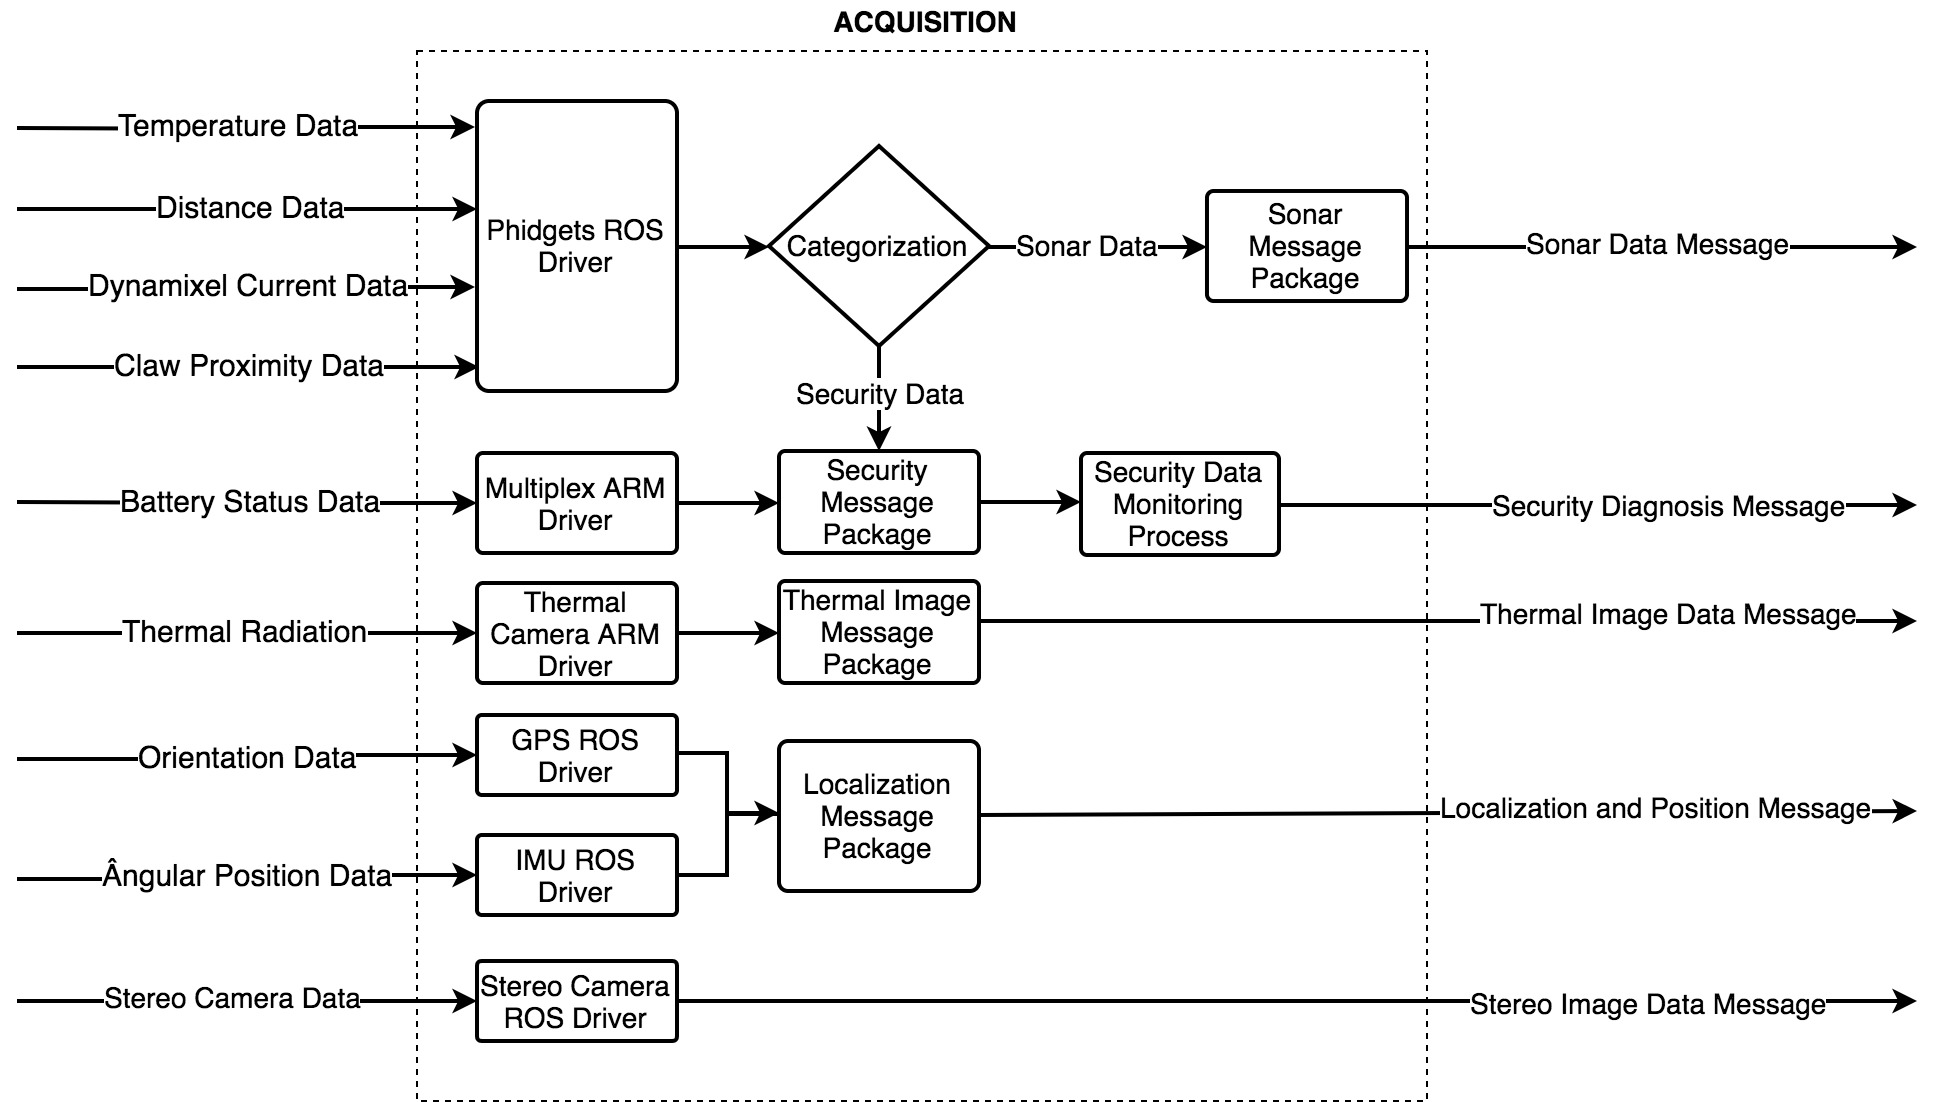
\includegraphics[height=7cm, width=14cm]{Fluxograma_Aquisition.jpg}
	\caption{Fluxograma da Funcionalidade Aquisição} \label{FuncAquisition}
	\end{figure}
	
      Para correta execução desta funcionalidade é necessário o funcionamento dos sensores segundo o nível de prioridade dos mesmos. Logo, um estudo de casos de falhas para cada sensor foi realizado, no qual foi definido um nível de criticidade de acordo com o impacto de sua função no sistema como um todo. Foram elaborados três níveis de criticidade:
     \begin{itemize}
     	\item Level 1 - Sensores com impacto crítico na operação. Em casos de falha, a inspeção não poderá ser realizada.
        \item Level 2 - Sensores com impacto médio na operação. Em caso de falha, a inspeção poderá ser realizada de forma parcial.
        \item Level 3 - Sensores com impacto leve na operação. Em caso de falha, não haverá dados de monitoramento da situação de temperatura e consuno energético do robô, porém a inspeção poderá continuar normalmente.
	\end{itemize}
	
	Na figura abaixo, pode-se observar os sensores e suas categorias.
	
	\begin{figure}[!ht]
	\centering
	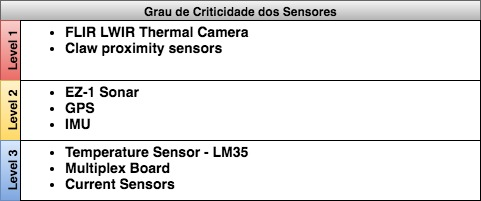
\includegraphics[height=7cm, width=14cm]{Figures/criticidade.jpg}
	\caption{Nível de criticidade dos sensores} \label{FuncAquisition}
	\end{figure}
	
	\subsubsection{Saídas}
     
     Esta funcionalidade possui quatro saídas:
     
    \begin{itemize}
        	\item Sonar Data Message: Mensagem de saída exclusiva para os dados do sonar EZ-1.
            \item Secutiry Diagnose Message: Mensagem contendo todos os dados relacionados à segurança e integridade do robô.
            \item Thermal Image Data Message: Mensagem exclusiva para os dados da câmera térmica.
            \item Localization and Position Message: Mensagem contendo os dados relacionados á localização e posicionamento angular do robô.
            \item Stereo Image Data Message: Mensagem exclusiva para os dados da câmera stereo.
        \end{itemize}
\pagebreak
\subsection{Localização}
\label{ssec:func2}
    \subsubsection{Objetivo}
        O objetivo desta funcionalidade é disponibilizar os dados de Localização do robô no ambiente ROS para a funcionalidade de Detecção.

    \subsubsection{Dependências}
        O sistema de localização depende dos dados de posicionamento e orientação disponibilizados pelo sistema de Aquisição.

    \subsubsection{Premissas}
        \begin{itemize}
         	\item O sistema de Aquisição deve está funcionando corretamente até o Nível 2 de criticidade dos sensores.
             \item GPS e IMU estão posicionados em uma estrutura rígida e com o menor vibração possível.
        \end{itemize}
        
    \subsubsection{Descrição da Funcionalidade}
        O sistema de localização envolve o monitoramento da posição latitudinal e longitudinal do robô, assim como a posição angular através do GPS e da IMU respectivamente.
        
        A localização é um package que ao receber uma requisição de informação, coleta os dados de posicionamento e orientação do robô provenientes do sistema de Aquisição e encaminha para o sistem que requisitou.
        
        O fluxograma deste funcionalidade pode ser visto na Figura \ref{fluxlocal}

        \begin{figure}[h!]
        	\centering
        	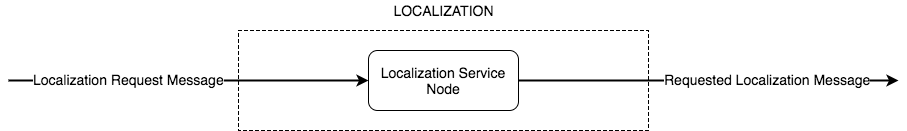
\includegraphics[width=16cm]{Fluxograma_Localization.png}
        	\caption{Fluxograma da Funcionalidade Localização} \label{fluxlocal}
    	\end{figure}
        \pagebreak
    \subsubsection{Saídas}

    \begin{itemize}
        	\item Requested Localization Message: Mensagem que informa os dados de localização para o sistema que os requisitou.
    \end{itemize}

    \subsection{Detecção}
\label{ssec:func3}

\subsubsection{Objetivo}

O objetivo desta funcionalidade é coletar as informações provinientes da câmera infravermelha e do sonar, como detectar a presença de pontos quentes e objetos presentes na área de servidão. Caso algum destes seja detectado, será enviado uma mensagem de alerta .

\subsubsection{Dependências}
 O sistema de detecção depende dos dados do sonar, frames da câmera térmica e frames da câmera stereo disponibilizados pelo sistema de Aquisição. Além disto, depende do sistema de Localização para adquirir informações de posicionamento e orientação do robô.

\subsubsection{Premissas}
\begin{itemize}
        	\item O sistema de Aquisição deve está funcionando corretamente até o Nível 2 de criticidade dos sensores.
            \item A câmera térmica deve estar calibrada e posicionada com ângulo de visão para as linhas de transmissão e seus obstáculos
            \item A câmera stereo deve está calibrada e posicionada com visada direta para os obstáculos.
            \item O sonar deve estar posicionado de forma a monitorar objetos abaixo da linha de transmissão.            
\end{itemize}

\subsubsection{Descrição da Funcionalidade}

A detecção é a funcionalidade responsável por identificar a presença de pontos quentes na linha de transmissão bem como de objetos na faixa de servidão. Ao identificar um destes elementos, o sistema solicita da funcionalidade de Localização os dados posicionamento e orientação do robô e envia uma mensagem de alerta.

A mensagem de alerta da detecção de um ponto quente informa a localização do robô e a localização do objeto no frame de imagem. Por isso recebe a mensagem de detecção de obstáculos. O package compara a região no frame de imagem da câmera stereo que contém o obstáculo com o frame da câmera IR com informação de ponto quente. 

A mensagem de detecção de objetos na faixa de servidão informa a distância da cota da linha até o objeto e a localização do mesmo. 

    \begin{figure}[!ht]
	\centering
	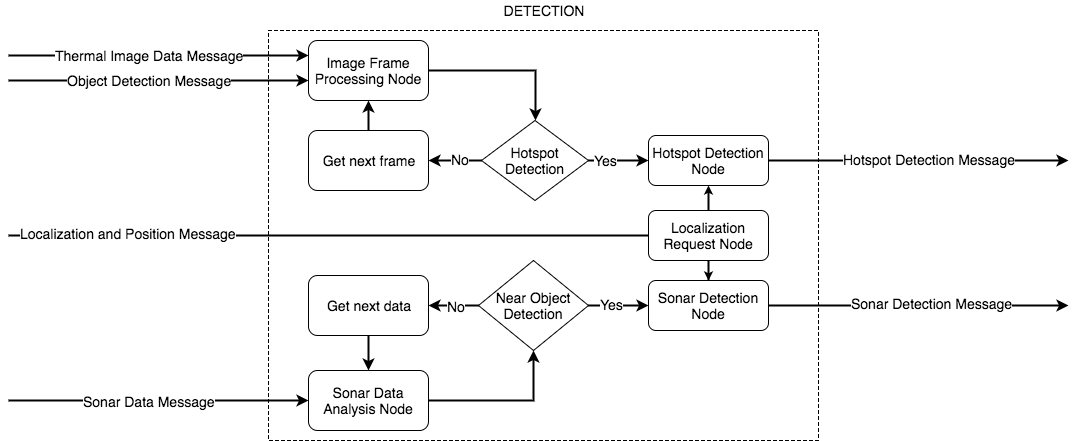
\includegraphics[width=16cm]{Fluxograma_Detection.png}
	\caption{Fluxograma da Funcionalidade Detecção} \label{FuncDetec}
	\end{figure}

\subsubsection{Saídas}

    \begin{itemize}
        	\item Hotspot Detection Message: Mensagem que informa a detecção de um ponto quente e informa a sua localização na imagem e localização do robô na linha.
            \item Sonar Detection Message: Mensagem que informa a detecção de objetos na faixa de servidão e sua localização na linha.
            %\item Localization Request Message: Mensagem de requisição dos dados posicionamento e orientação do robô para o sistema de Localização
    \end{itemize}
    \pagebreak

%--------- NEW SECTION ----------------------
\section{Interface do Usuário}
\label{sec:ui}
    \begin{figure}[!ht]
	\centering
	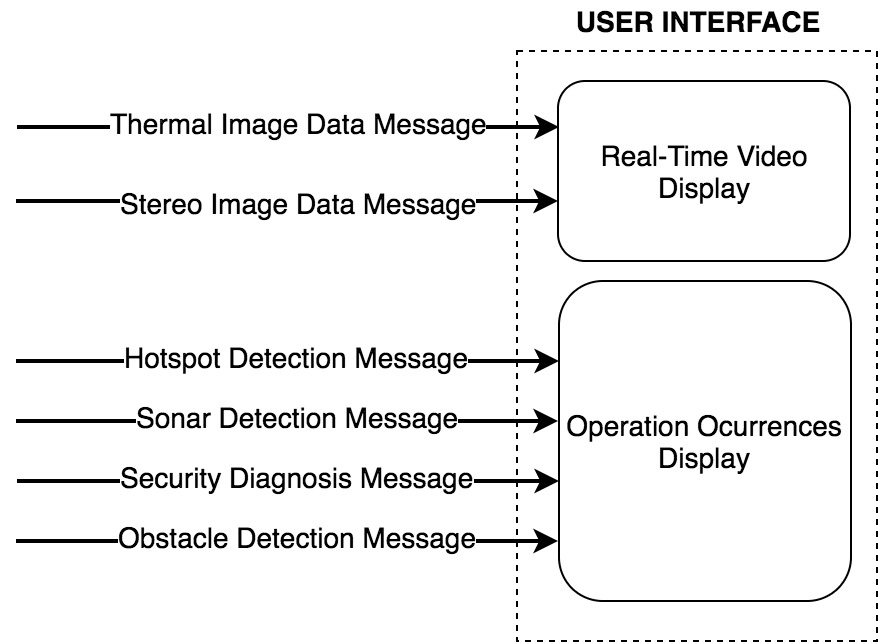
\includegraphics[width=16cm]{Figures/Fluxograma_Interface.jpg}
	\caption{Fluxograma da Interface do Usuário} \label{UI}
	\end{figure}
	


\pagebreak
\newpage
%--------- NEW SECTION ----------------------
%\section{Simulação do sistema}
%\label{sec:sim}
%asdfadsfsdfs


